% Options for packages loaded elsewhere
\PassOptionsToPackage{unicode}{hyperref}
\PassOptionsToPackage{hyphens}{url}
%
\documentclass[
]{article}
\usepackage{amsmath,amssymb}
\usepackage{lmodern}
\usepackage{ifxetex,ifluatex}
\ifnum 0\ifxetex 1\fi\ifluatex 1\fi=0 % if pdftex
  \usepackage[T1]{fontenc}
  \usepackage[utf8]{inputenc}
  \usepackage{textcomp} % provide euro and other symbols
\else % if luatex or xetex
  \usepackage{unicode-math}
  \defaultfontfeatures{Scale=MatchLowercase}
  \defaultfontfeatures[\rmfamily]{Ligatures=TeX,Scale=1}
\fi
% Use upquote if available, for straight quotes in verbatim environments
\IfFileExists{upquote.sty}{\usepackage{upquote}}{}
\IfFileExists{microtype.sty}{% use microtype if available
  \usepackage[]{microtype}
  \UseMicrotypeSet[protrusion]{basicmath} % disable protrusion for tt fonts
}{}
\makeatletter
\@ifundefined{KOMAClassName}{% if non-KOMA class
  \IfFileExists{parskip.sty}{%
    \usepackage{parskip}
  }{% else
    \setlength{\parindent}{0pt}
    \setlength{\parskip}{6pt plus 2pt minus 1pt}}
}{% if KOMA class
  \KOMAoptions{parskip=half}}
\makeatother
\usepackage{xcolor}
\IfFileExists{xurl.sty}{\usepackage{xurl}}{} % add URL line breaks if available
\IfFileExists{bookmark.sty}{\usepackage{bookmark}}{\usepackage{hyperref}}
\hypersetup{
  pdftitle={Final Project: Regression From The Mean},
  pdfauthor={Zhengtao Xu, Jennings Cheng and Collin Carmichael},
  hidelinks,
  pdfcreator={LaTeX via pandoc}}
\urlstyle{same} % disable monospaced font for URLs
\usepackage[margin=1in]{geometry}
\usepackage{graphicx}
\makeatletter
\def\maxwidth{\ifdim\Gin@nat@width>\linewidth\linewidth\else\Gin@nat@width\fi}
\def\maxheight{\ifdim\Gin@nat@height>\textheight\textheight\else\Gin@nat@height\fi}
\makeatother
% Scale images if necessary, so that they will not overflow the page
% margins by default, and it is still possible to overwrite the defaults
% using explicit options in \includegraphics[width, height, ...]{}
\setkeys{Gin}{width=\maxwidth,height=\maxheight,keepaspectratio}
% Set default figure placement to htbp
\makeatletter
\def\fps@figure{htbp}
\makeatother
\setlength{\emergencystretch}{3em} % prevent overfull lines
\providecommand{\tightlist}{%
  \setlength{\itemsep}{0pt}\setlength{\parskip}{0pt}}
\setcounter{secnumdepth}{-\maxdimen} % remove section numbering
\ifluatex
  \usepackage{selnolig}  % disable illegal ligatures
\fi

\title{Final Project: Regression From The Mean}
\author{Zhengtao Xu, Jennings Cheng and Collin Carmichael}
\date{8/6/2021}

\begin{document}
\maketitle

\textbf{Section 1: Introduction}

In this project we are going to construct models to predict PM2.5 in
Beijing, China. Beijing and lots of part of China is experiencing
chronic air pollution, and the main pollutants are PM 2.5 {[}1{]}. PM
2.5 refers to airborne particles with diameter less than 2.5 μm {[}1{]}.
Studied has shown that breathing excessive PM 2.5 is harmful to lung,
and is a cause to serious respiratory and cardiovascular diseases, and
even the death {[}1{]}. Moreover, China's State Council has enacted the
target to reduce PM 2.5 by 25 percent from 2012 to 2017 for Beijing, and
the statistic approach of predicting PM 2.5 is not only helpful to
determine the goal of decreasing PM 2.5, but also necessary to predict
the harmful PM 2.5 level in Beijing, in order to protect people's health
{[}1{]}.

Data mainly comes from two sources, the US embassy in Beijing, located
(116.47 E, 39.95 N), and hourly meteorological measurements at Beijing
Capital International Airport (BCIA), obtained from weather.nocrew.org
{[}1{]}. Though two places are 17 kilometers apart, they share nearly
identical weather condition {[}1{]}. These data set includes PM2.5 (fine
particulate matter), concentrations with a number of meteorological
variables for the city of Beijing during the 1st January 2010 to the
31st December 2014 {[}1{]}. The Airport's data is mainly used to
calibrate with the embassy data {[}1{]}.

To achieve the prediction goal, we will first conduct the EDA analysis,
in this part we will summary the basic statistics on the time series of
PM2.5 data, as well as the relevant impact factor or signal factors and
their relationships with each other.

After this, the we will construct prediction models, from multiple
linear regression to generalized least squares and choose the model that
can achieve the regression assumptions of constant variance as well as
normal residual. Finally, we will summarize results and explain why our
model was effective and what impact this has on response.

\textbf{Section 2: Exploratory Data Analysis}

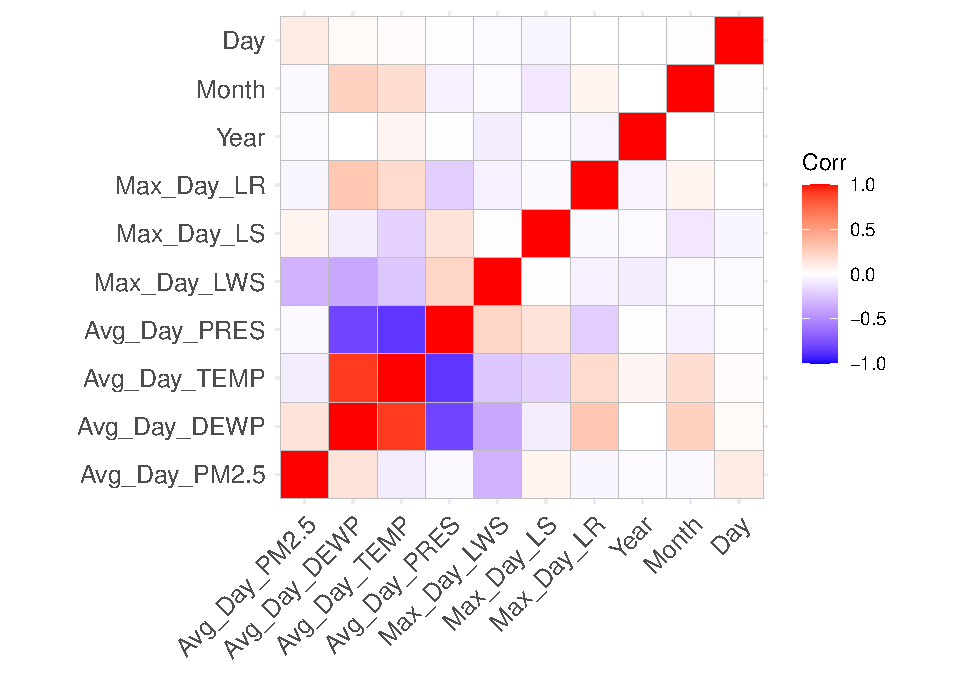
\includegraphics{Final_Project_2_files/figure-latex/unnamed-chunk-3-1.pdf}
Looking at a correlation heatmap we see aside from dewpoint
precipitation and temperature there are no significant correlation in
other variable

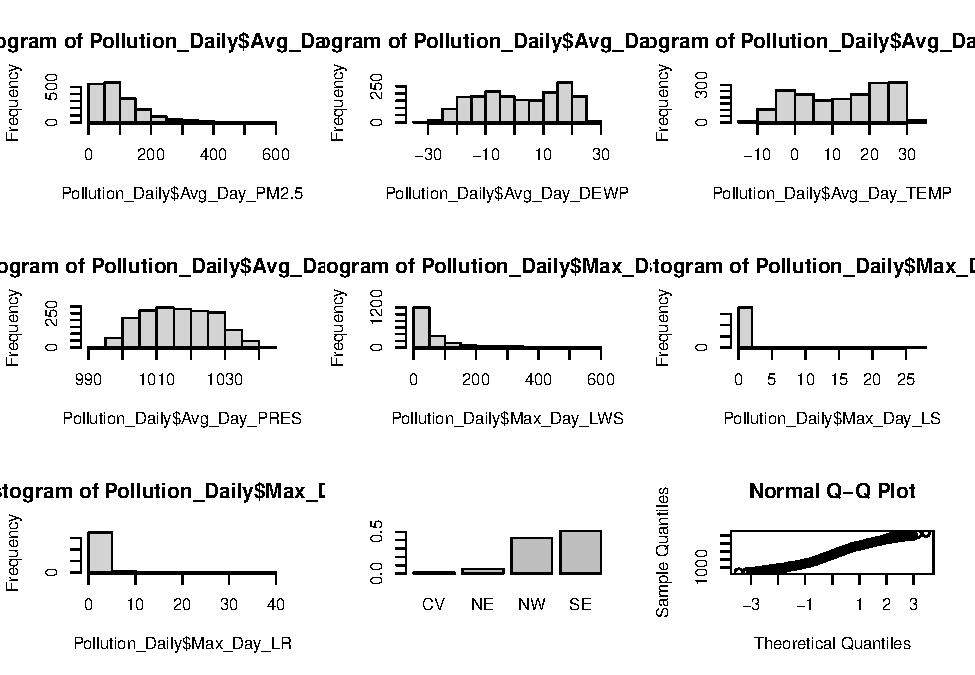
\includegraphics{Final_Project_2_files/figure-latex/unnamed-chunk-4-1.pdf}
We can see that PM2.5 has an inverse distribution with values skewed
towards low PM2.5 but many high values that go beyond the median

Temp and Dew point are highly related and so may not need to be included
in the same model

Precipitation looks like a bell curve but not normal as seen in the plot
in 3,3

Wind speed is similar but not identical to PM2.5 in that it has an
inverse distribution so it may be highly important in prediction

There is almost always not any snow in Beijing and the max is 27 for a
day

Rain is also infrequent but there are times when there is a lot of rain
so we may assume that rain and snow are not the same

The most common direction is SE and NW while sometimes NE or CV

Now that we know the distributions we can take a look at some pm2.5 vs
predictor

The pm and time is not a clear relationship and there are many seasonal
spikes - One thing is that since there are random fluctations in our
final model we will not use Date since in a regression model the advance
of one day would theoretically advance pm2.5 which is not the
relationship we see - and also any hypothesize increase in pm2.5 due to
global warming trends in the date would be explained by the year
variable and of course the other predictors so we decide not to use the
column for our analysis. In the same way we would make month and day
factors due to the same concern which is an increase in either of these
do not necessarily mean an increase in particulate.

We can also extract that dew, temp, pres are very clearly related from
the following which corroborates what was shown in heatmap.

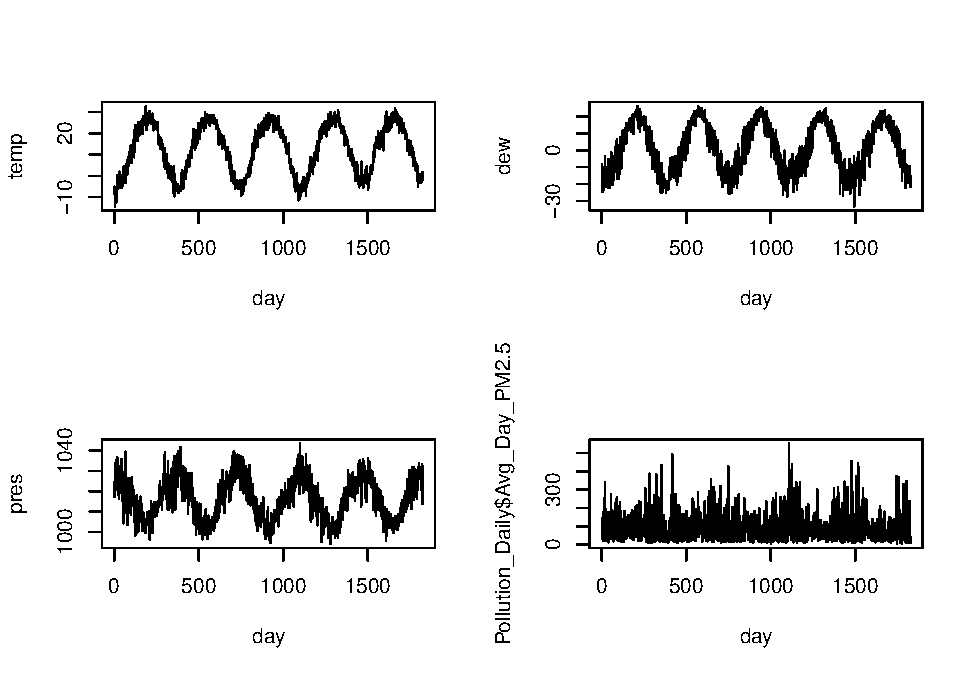
\includegraphics[height=0.9\textheight]{Final_Project_2_files/figure-latex/unnamed-chunk-5-1}

PM2.5 is obviously highly unpredictable from just looking at the time
series. We will see if there is a relationship with day or month so that
we can see if including these in the linear regression as factor would
make sense.

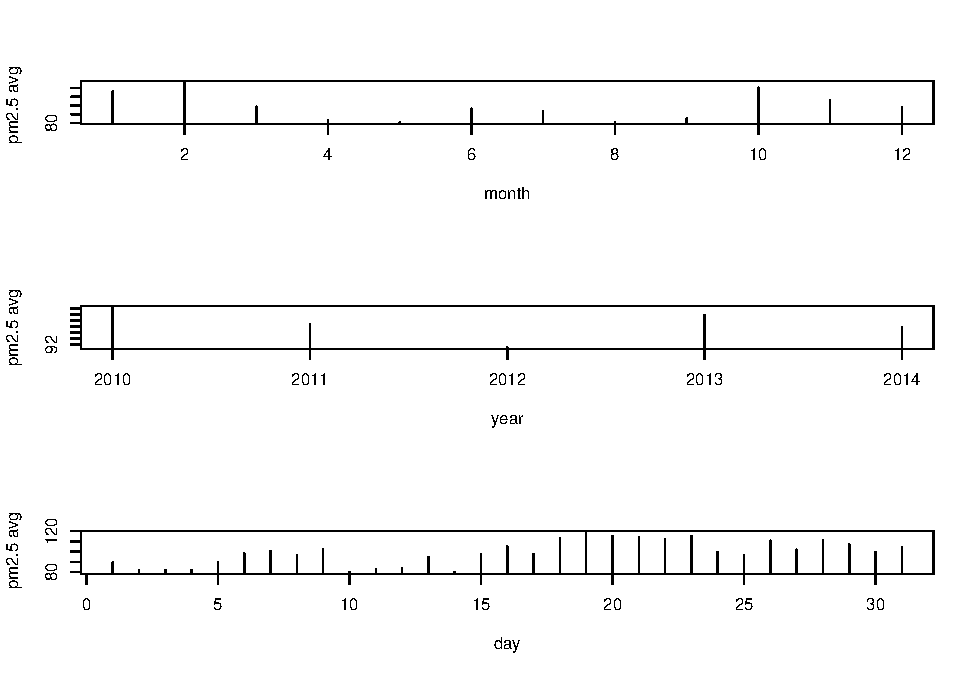
\includegraphics{Final_Project_2_files/figure-latex/unnamed-chunk-6-1.pdf}
As we see the variation between the month year and day is important -
highly significant differences between different days, years, or months
so it would make much sense to include these in MLR

\textbf{3.1: Fitting model and diagnostic}

Now that we know what our data looks like in accordance with the
response we can fit a multiple linear regression with response
Avg\_Day\_PM and predictor every variable besides `Date\_D', and look at
the results. We can also see the predicted values of pm2.5 in in red on
the testing (every 5th observation in the 5 year long data set) after
fitting on the training dataset(which is the complement of test)

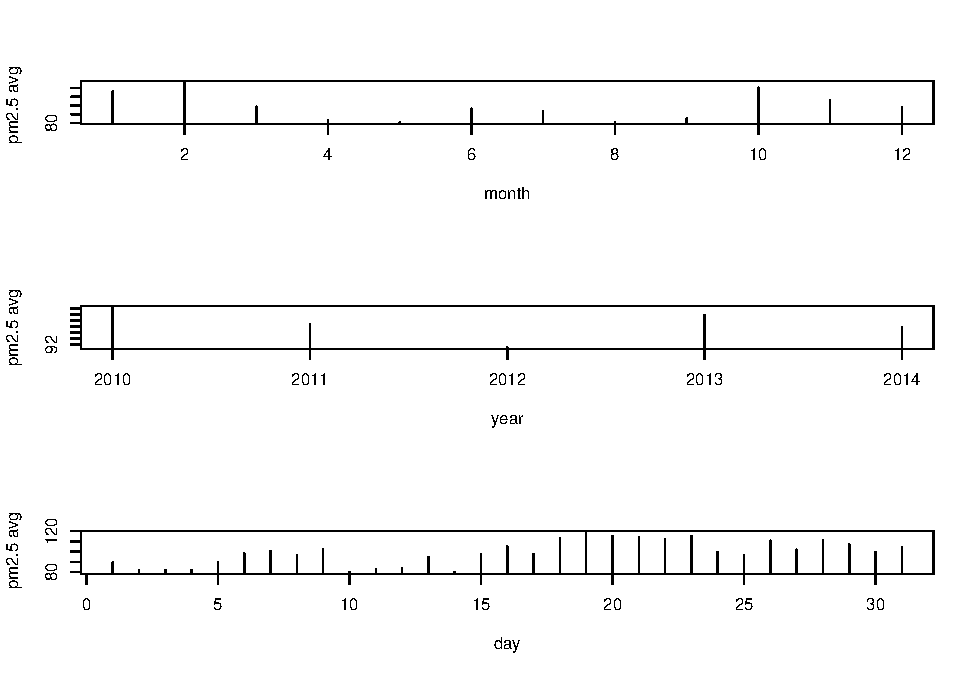
\includegraphics{Final_Project_2_files/figure-latex/unnamed-chunk-7-1.pdf}

\begin{verbatim}
## $adj.r.squared
## [1] 0.4862557
\end{verbatim}

After fitting a full model with every predictor besides `Date\_D' and
Month, Year, and Day all in factor version we see that firstly there are
many insignificant predictors unsurpisingly in the factors. As expected
we see highly significant predictors in the factor(Day) in the 20s since
that is what we saw highly in the mean particulate vs.~day
visualization. But the majority of days are insignificant so it makes
sense to just drop the day column. Every month factor is significant
besides the 2nd so this is important to keep. Year is all insignificant
unless the year is 2012, which means 2012 is a lower pm anomaly. We
could hypothetically exclude every non 2012 level but the simpler way is
to not use the predictor.

Before considering dropping variables we need to check diagnostics. So
here are some of the important assumptions that we will have to
validate, namely constant variance, non correlated and normal residuals.

We can also check the visualizations for the regression of normality and
heteroscedasticity.

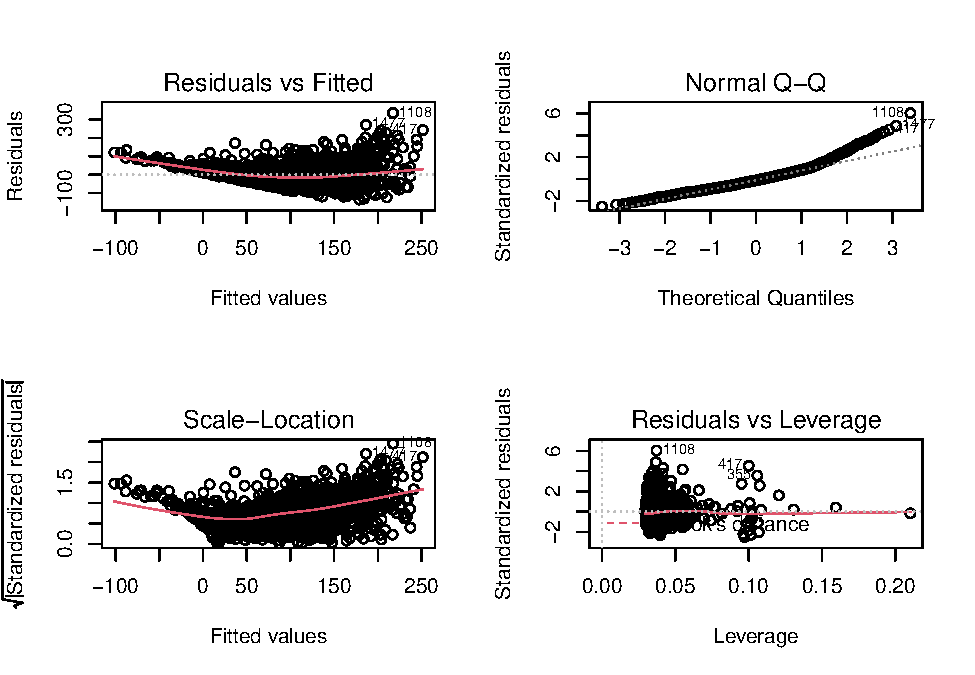
\includegraphics{Final_Project_2_files/figure-latex/unnamed-chunk-9-1.pdf}
Taking a glance at our linear model, we see that it does not appear to
meet all error assumptions. Particularly, the Q-Q plot suggests
non-normality and the Fitted-Residual plot suggests heteroscedasticity
and some degree of non-linearity. The Residuals-Leverage plot however
appears to indicate we don't have highly influential points.

\begin{verbatim}
##       bptest p shapiro test p durbin watson p
## 1 3.392827e-24    4.94394e-23    1.493388e-70
\end{verbatim}

As we can tell through testing more formally, none of the error
assumptions of homocedasticity, normality, and uncorrelated errors are
accurate.

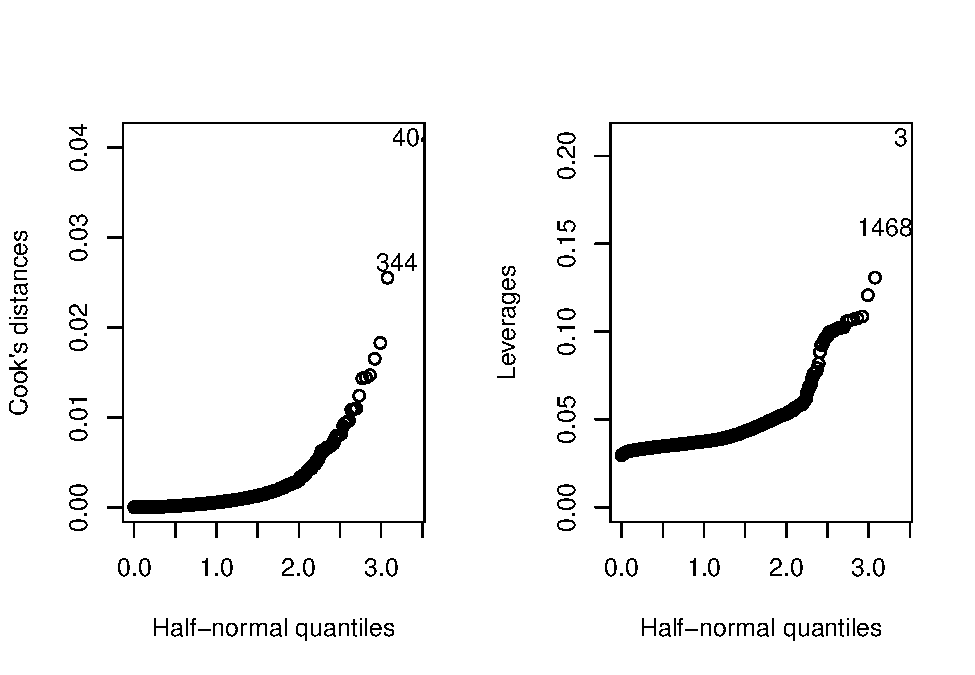
\includegraphics{Final_Project_2_files/figure-latex/unnamed-chunk-11-1.pdf}
In regards to unusual observations, our maximum cooks distance as seen
above indicates we have no datapoints that would be classified as highly
influential, since it is much less than one. In constrast, however, we
seem to have an abundance of high-leverage points. However, it is
unclear at first glance how many of these are ``good'' or ``bad''
leverage points, although we can assume some points like observations 3
and 1468 with wildly different y-values are likely ``bad.''

\begin{verbatim}
##             b d        c
## 417  4.541472 > 4.152753
## 1108 6.105989 > 4.152753
## 1125 4.181143 > 4.152753
## 1477 4.915473 > 4.152753
## 1517 4.338133 > 4.152753
\end{verbatim}

As we can see above, we also have four outliers in training data.

All things aside, in order to remedy non linearity, heteroscedasticity,
non normal residual and autocorrelation we can apply a Boxcox
transformation first for non linearity and making normally distributed
residuals:

This is the maximum likelihood for lambda so that will be the
transformation we use

We fit the model with the boxcox transformation which involves applying
the transformation responseNew=(responseOld\^{}lambda-1)/lambda

\begin{verbatim}
##   R-square value     bptest p shapiro test p durbin watson p
## 1      0.5892627 0.0003424676      0.5473221    1.497302e-57
\end{verbatim}

The shapiro wilk shows that we easily have residual normal with p=0.54
\textgreater.05 while we see that there is autocorrelation via dwtest
and heteroscedasticity which is improve - R squared also went up by a
massive \textasciitilde0.1 which means the variation we explain has
increased substantially

So our explanation of variation improved but there is still steep
autocorrelation and heteroscedasticity - we could combine Generalised
Least Squares with correlated error to our Boxcox transformed data for
the first one and try a different model with OLS and the Boxcox
transformation and evaluate the performance of both model:

\begin{verbatim}
##   transormed only r-mse GLS Transformed r-mse original model r-mse
## 1              51.33086              52.18969             51.70159
\end{verbatim}

\begin{verbatim}
## $corStruct
##         lower      est.    upper
## Phi 0.4397209 0.4903428 0.537859
## attr(,"label")
## [1] "Correlation structure:"
\end{verbatim}

\begin{verbatim}
##   original aic   box aic gls with transformed aic
## 1     11631.74 -537.3763                 3209.409
\end{verbatim}

As we can see after applying a Generalised Least Square with correlated
error with boxcox transformation we have an rmse of 52, which is
slightly higher than the original and only transformed linear
regression. Also we see that we cannot reject the null hypothesis of
residual being correlated since the lower bound of Phi which is the
correlation variable does not include 0 which is what we would need to
reject the null hypothesis. This suggests that GLS may not be the best
model for this data since there is still correlation and the r-mse is
higher than OLS

Therefore, it may be a good idea to stick with OLS specifically the
transformed regression for the sake of fitting a parametric model in
this dataset.

\begin{verbatim}
##        rmse   bptest p shapiro p        aic
## BP 114.4869 0.01446565  0.2985939 -38.51955
\end{verbatim}

We see that this model has normal residual as well as
heteroscedasticity. However there is autocorrelation so a non parametric
method such as regression splines or kernel estimation may be a better
way to model particulates in Beijing though our model is greatly
improved from the previous.

\textbf{Section 4: Conclusions}

Through our analysis we have learned many things, such as: Through
analyzing the data we were able to find out several things about this
dataset. We were able to find correlation between several of the
meteorological variables used, with dew point, temperature, and pressure
all being somewhat highly correlated. This is hardly a surprising
phenomenon to anyone who has studied physics or chemistry, and this
fact, while complicated from a data analysis point of view, lends
credibility to the accuracy of the model.

Likewise, we noted that the original dataset: pollution, and the dataset
output from the useful code provided by the class instructor:
pollution\_daily, both have multiple variables through which they
represent time, including the month, year, and day variables. Having an
additional variable like Date\_D then would obviously cause more issues
in regards to correlation.

Through diagnostic testing, we were able to tell that the initial full
model described by the project instructions did not meet the error
assumptions of homoscedasticity, normality, and had autocorrelation.
Furthermore, in our train dataset we found many unusual observations,
with most being high leverage points, and none being high influence
points. Four outliers were found within the train dataset and two were
found within the test dataset, however, we decided it would not make
sense to remove data from the final dataset to test our model, so we did
not in this case.

In order to fix our error assumptions, we first performed a box cox
transformation on the original full model. We found that R squared
increased by a gigantic 0.1 which meant our model explained the
variation in particulates much better than the non transformed data.
Through this we met the model assumption of residuals being normal.
There was still heteroscedasticity and errors correlation. So we decided
to use Generalised Least Squares for this.

Our model was worse using gls and from the phi interval we did not
reject the hypothesis that there is autocorrelation, therefore we
switched to back to a simple boxcox transformation. However we also saw
in the gls model that shows our model fits the dataset more precisely,
and of course it also looks better under diagnostics.

To sum up in bullet points: Original Predictors Show Significant
Correlation Full Model Does Not Meet Error Assumptions/Has Unusual
Observations Doing generalised least squares did not improve the model
Final Model which is a boxcox transformation with factor day, month,
year predicts PM2.5 Better Than Full Model

\end{document}
